\documentclass{standalone}
\usepackage{tikz}
\usepackage{ctex,siunitx}
\setCJKmainfont{Noto Serif CJK SC}
\usepackage{tkz-euclide}
\usepackage{amsmath}
\usepackage{wasysym}
\usetikzlibrary{patterns, calc}
\usetikzlibrary {decorations.pathmorphing, decorations.pathreplacing, decorations.shapes,}
\begin{document}
\small
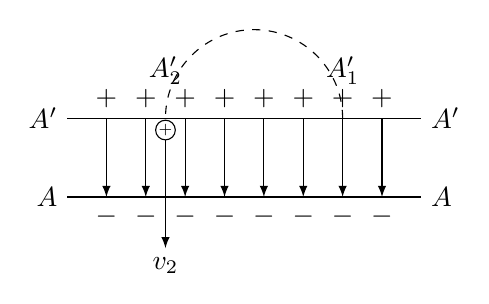
\begin{tikzpicture}[>=latex,scale=0.5]
  \useasboundingbox(-1,4.3)rectangle(10,-2);
  \draw (0,0)node [left]{$A$}--(9,0)node [right]{$A$};
  \draw (0,2)node [left]{$A'$}--(9,2)node [right]{$A'$};
  \foreach \x in {1,2,...,8}
  {
      \draw [<-](\x,0)--(\x,2);
     \node at (\x, 2.5){$+$};  \node at (\x, -.5){$-$};
  }
  \draw [dashed] (7,2) arc (0:180:2.25);	
  \draw (2.5,2-.3) circle (.25) node {\tiny +};
  \node at (2.5,2)[above =3mm]{$A'_2$}; 
  \node at (7, 2)  [above =3mm]{$A'_1$};
  \draw [->](2.5,2-.55)-- (2.5,-1.3)node[below]{$v_2$};	
\end{tikzpicture}
\end{document}